%!TEX root = ms.tex
\section{Best orthogonalized subset selection (BOSS)}
\label{sec:boss}

For predictors in general position, BS is not computationally feasible for large problems. In this section, we propose a feasible LS-based subset selection method BOSS that is based on orthogonalizing the predictors. The orthogonalization not only makes the computation of BS feasible, but also allows us to take advantage of the superior performance of AICc-hdf as discussed in Section \ref{sec:aicc_performance_bs}. BOSS using AICc-hdf as the selection rule has computational cost of the order $O(npK)$, that is of the same order as a multiple regression on all $p$ predictors for the problem where $n>p$, and on a selected subset of $n$ predictors for $n \le p$. We further demonstrate the competitive performance of BOSS via simulations and real world examples. 

The main steps for BOSS can be summarized as follows: 1) order and orthogonalize the predictors, 2) perform BS on the set of orthogonalized predictors, 3) transform the coefficients back to the original space, and 4) use a selection rule such as AICc-hdf to choose the optimal single subset. 

\subsection{The solution path of BOSS}
\label{sec:boss_solutionpath}

BOSS starts by ordering and orthogonalizing the predictors, taking $K$ steps in total. The ordering is based on partial correlations with the response $y$, and the orthogonalization is based on QR decomposition with Gram-Schmidt. For step $k$, we use $X_{S_{k-1}}$ to denote the set of ordered predictors from the previous step, and use $Q_{S_{k-1}}$ to denote the orthogonal basis of $X_{S_{k-1}}$. From the remaining $p-k+1$ predictors, we choose the one that has the largest correlation with $y$ conditioning on $Q_{S_{k-1}}$, that is the correlation between $y$ and the residual from regressing a candidate predictor on $Q_{S_{k-1}}$. This costs $O(n)$ since we maintain the regression result, e.g. estimated coefficients and residual, in the previous steps. Repeating the above step for all $p-k+1$ predictors costs $O(n(p-k+1))$. We then update the QR decomposition, by adding the chosen predictor as a new column, which costs $O(n(K-k))$ via the modified Gram-Schmidt algorithm as discussed in \citet{hammarling2008updating}. After $K$ steps, we end up with an ordered set of predictors $X_{S_K}$ and its orthogonal basis $Q_{S_K}$, and the total cost for ordering and orthogonalization is $O(npK)$. We denote the regression coefficient vector of $y$ on $Q_{S_K}$ as $z$. BOSS then performs BS on $Q_{S_K}$, which is a ranking of predictors based on their absolute values of corresponding element in $z$, and the cost is $O(K\log(K))$. We use $\tilde{\gamma}(k_Q)$ to denote the BS coefficient vector at size $k_Q$, where $k_Q=1,\cdots,K$ specifies the subset size in the orthogonal space. Finally, BOSS transforms the coefficient vectors $\tilde{\gamma}=[\tilde{\gamma}(0),\cdots,\tilde{\gamma}(K)]$ back to the original space. Therefore, the total cost for the entire solution path of BOSS is on the order of $O(npK)$. The detailed implementation for obtaining the solution path is summarized as steps 1-5 in Algorithm \ref{alg:boss}.

% main algorithm
\begin{algorithm}
	\caption{Best Orthogonalized Subset Selection (BOSS)}\label{alg:boss}
	\begin{enumerate}[label=\arabic*.]
		\item Standardize $y$ and the columns of $X$ to have mean $0$, and denote the means as $\bar{X}$ and $\bar{y}$.
		%\item Denote $S_k$ as the set of predictors that are active at step $k$ and let $S={1,\cdots, p}$.

		\textbf{Order and orthogonalize the predictors:}

		\item From the $p$ predictors, select the one that has the largest marginal correlation with the response $y$,  and denote it as $X_{S_1}$. Standardize $X_{S_1}$ to have unit $l_2$ norm and denote it as $Q_{S_1}$, where $S_1$ is the variable number of this chosen predictor. Calculate $R_{S_1}$ such that $X_{S_1} = Q_{S_1} R_{S_1}$. Let $S=\{1,\cdots, p\}$. Initialize vectors $\text{resid}_j=X_j$ where $j=1,\cdots,p$.
		\item For $k=2,\cdots,K$ ($K=\min\{n,p\}$):
		\begin{enumerate}[label=\alph*.]
			\item For each of the $p-k+1$ predictors $X_j$ in $X_{S \setminus S_{k-1} }$, calculate its partial correlations with the response $y$ conditioning on $Q_{S_{k-1}}$. 
			\iffalse
			\begin{enumerate}[label=a\arabic*.]
				\item Regress $y$ on $q$, augment $Z$ with the coefficient $z$. Set $\text{resid1} = \text{resid1} - zq$.
			\end{enumerate}
			\fi
			%\begin{enumerate}[resume*,label=a\arabic*.]
			\begin{enumerate}[label=a\arabic*.]
				%\item Regress $x_j$ on $q$, call the coefficient $r$. Set $\text{resid2}_j = \text{resid2}_j - rq$.
				%\item Calculate the correlation between resid1 and $\text{resid2}_j$.
				\item Regress $X_j$ on $Q_{S_{k-1} \setminus S_{k-2}}$ ($S_{k-2}=\emptyset$ if $k=2$), and denote the estimated coefficient as $r$. Update $\text{resid}_j = \text{resid}_j - r Q_{S_{k-1} \setminus S_{k-2}}$.
				\item Calculate the correlation between y and $\text{resid}_j$.
			\end{enumerate}
			\item Select the predictor that has the largest partial correlation in magnitude, augment $S_{k-1}$ with this predictor number and call it $S_{k}$.
			\item Update $Q_{S_{k-1}}$ and $R_{S_{k-1}}$ given the newly added column $X_{S_k \setminus S_{k-1}}$, and call them $Q_{S_k}$ and $R_{S_k}$. The update is based on the modified Gram-Schmidt algorithm as discussed in \citet{hammarling2008updating}.
		\end{enumerate}
		
		\textbf{BS on the orthogonalized predictors $Q_{S_{K}}$:}

		\item Calculate $\tilde{\gamma}_j (k_Q)= z_j \mathbbm{1}(|z_j| \ge |z_{(k_Q)}|)$, i.e. the $j$-th component of coefficient vector for subset size $k_Q$, where $z=Q_{S_{K}}^T y$ and $z_{(k_Q)}$ is the $k$-th largest entry in absolute values. Let $\tilde{\gamma} = [\tilde{\gamma} (0) \tilde{\gamma} (1) \cdots \tilde{\gamma} (K)]$.
		
		\textbf{Transform back to the original space:}

		\item Project $\tilde{\gamma}$, a $p \times (K+1)$ matrix, to the original space of $X_{S_{K}}$, i.e. back solving $R \tilde{B} = \tilde{\gamma}$, and re-order the rows of $\tilde{B}$ to their correspondences in $X$, i.e. $\hat{B} = O \tilde{B}$ where $O$ represents the ordering matrix s.t. $X_{S_{K}}=XO$. The intercept vector is $\hat{B}_0 = \bar{y} \mathbbm{1} - \hat{B}^T \bar{X}$. 

		\textbf{Select the subset:}

		\item Select the subset using AICc-hdf (replacing edf with hdf in \eqref{eq:aicc_edf}), where hdf is calculated via Algorithm \ref{alg:hdf}, by inputting $(Q_{S_{K}},\hat\sigma,\hat\mu)$. For $n > p$, we use OLS estimates based on the full model, i.e. $\hat{\mu}=Q_{S_{K}} z$, $\hat{\sigma}^2 = \lVert y-\hat{\mu} \rVert_2^2/(n-p)$. For $n \le p$, we use $\hat{\mu}=\hat{\mu}_l$ and $\hat{\sigma} = \sqrt{\lVert y-\hat{\mu}_l \rVert_2^2 / (n-\text{df}(\hat{\mu}_l)-1)}$ as discussed in \citet{reid2016study}, where $\hat{\mu}_l$ are the lasso fitted values based on 10-fold CV and df$(\hat{\mu}_l)$ is the corresponding number of non-zero coefficients in the lasso estimate. Note that the inclusion of an intercept term implies that hdf is increased by $1$. 
	\end{enumerate}
\end{algorithm}


The ordering of predictors is an important part of implementation of the algorithm. Consider a sparse true model with only two uncorrelated predictors $X=[X_1,X_2]$, $\beta=[0,1]^T$ and a high SNR. The best model in such a scenario is LS regression on $X_2$. Without the ordering step, the orthogonal basis is $Q=[Q_1,Q_2]$ s.t. $X=QR$, i.e. the predictors are orthogonalized in their physical orders. The one-predictor model ($k_Q=1$) of BS can either be $Q_1$ or $Q_2$, which when transformed back to the space of $X$ do not correspond to LS regression upon $X_2$. The former corresponds to LS estimates upon $X_1$, while the latter is a linear combination of LS estimates upon $X$ and LS estimates upon $X_1$; the former leads to a completely wrong model while the latter results in non-zero coefficients on both predictors. In contrast, if $X_2$ is the first variable orthogonalized, the best subset will be based on that variable alone, the correct choice. Therefore, the ordering step is crucial to both sparsity as well as predictive performance. It is worth noting that BOSS is flexible in terms of the choice of ordering rules. For instance, a less aggressive rule based on the lars algorithm \citep{efron2004least} could be adopted instead. We leave discussion of the benefits and drawbacks of different ordering rules to future work. Note that we show that the coefficients of BOSS can be expressed as a linear combination of the LS coefficients on subsets of $X$ in Theorem \ref{thm:correspondence}, the proof of which can be found in the Supplemental Material Section \ref{sec:correspondence}. 


\begin{theorem}[Coefficients of BOSS are a linear combination of LS coefficients on subsets of $X$] 
	Suppose $X$ has full column rank and the columns are already ordered, i.e. $X=X_{S_{K}}$. $X=QR$ where $Q$ is an $n \times K$ matrix with orthonormal columns and $R$ is a $K \times K$ upper-triangular matrix. Let $S_k=\{j_1,j_2,\cdots,j_{k_Q}\}$ denote the support (position of predictors) of the best $k_Q$-predictor model given by BS upon $(Q,y)$, and use $\hat{\gamma}(k_Q)$ ($K$ by $1$) to denote the BS coefficients. The corresponding coefficients in the $X$ space, i.e. $\hat{\beta}(k_Q)$ s.t. $R\hat{\beta}(k_Q)=\hat{\gamma}(k_Q)$, can be expressed as
	\begin{equation*}
	\hat{\beta}(k_Q) = \sum_{j\in S_k} \left(\hat{\alpha}^{(j)} - \hat{\alpha}^{(j-1)}\right),
	\end{equation*}
	where the first $j$ entries in $\hat{\alpha}^{(j)}$ ($K$ by $1$) are LS coefficients of regressing $y$ upon $[X_1,X_2,\cdots,X_j]$ (the first $j$ columns in $X$), and the remaining $K-j$ entries are zero.

	\label{thm:correspondence}
\end{theorem}

\subsection{Connection to FS and the advantage of BOSS}

BOSS is closely related to FS. In fact, instead of performing BS on the set of orthogonalized predictors $Q_{S_{K}}$ in the fourth step of Algorithm \ref{alg:boss}, if we fit LS on the subset of $Q_{S_{K}}$ in a nested fashion, i.e. $\tilde{\gamma}_j (k_Q)= z_j \mathbbm{1}(j \le k_Q)$ and $z=Q_{S_{K}}^T y$, steps 1-5 of the algorithm provide the solution path of FS, and is similar to the orthogonal greedy algorithm discussed in \citet{ing2011stepwise}. Since BS on orthogonal predictors $Q_{S_K}$ is essentially ranking the predictors based on their LS coefficients ($O(K\log(K))$ operations), BOSS involves little additional computational cost compared to FS.

BOSS can, however, provide a better solution path than FS. At a given step, once a predictor is selected, it remains in the subsets of every following step of FS. In many circumstances, the greedy characteristic can lead to overfit, since noise predictors (those with $\beta_j=0$) step in during early steps. However, BS on the set of orthogonalized predictors gives the chance for BOSS to ``look back'' at the predictors that are already stepped in. By revisiting these predictors and allowing them to be dropped, BOSS can provide a solution path that is sparser, with better predictive performance compared to FS. 

We consider two numerical examples Sparse-Ex3 and Sparse-Ex4, where the true models are sparse. The true coefficient vectors for Sparse-Ex3 and Sparse-Ex4 are $\beta=[1_6,0_{p-6}]^T$ and $\beta=[1,-1,5,-5,10,-10,0_{p-6}]^T$, respectively. We consider a high SNR and a high correlation between predictors ($\rho=0.9$). For Sparse-Ex3, the signal predictors (those with non-zero coefficients) are pairwise correlated with noise predictors (correlation coefficient is denoted as $\rho$), while for Sparse-Ex4, the signal predictors are pairwise correlated with opposite effects. We generate the design matrix $X$ once, and draw $1000$ replications of the response $y$ based on \eqref{eq:truemodel_def}. The details of the model setup are given in Supplemental Material Section \ref{sec:simulation_setup_generalx}.

Figure \ref{fig:lossratio_fs_boss_k} shows the average RMSE along the solution paths of BS, FS and BOSS, for the two examples. When the true model is Sparse-Ex3, all three methods provide almost the same solution path. However, for Sparse-Ex4, we see a clear advantage of BOSS over FS in early steps up until about the fifteenth step. Recall that in Sparse-Ex4, there are $p_0=6$ predictors with $\beta_j \ne 0$ that are pairwise correlated with opposite effects, where each pair together leads to a high $R^2$ but each single one of them contributes little. When the correlation between the variables is high, the effect of one almost completely cancels out the effect of the other on $y$. Therefore all of the predictors (both true and noise predictors) have approximately zero marginal correlation with $y$, and they have equal chance of stepping in. Since the subsets along the solution path of FS are nested, if a noise predictor steps in during early steps, it remains in the subsets of every following step, and hence the subset containing both variables in the pair may appear in a late stage. In contrast, BOSS takes ordered predictors provided by FS, and re-orders them by performing BS upon their orthogonal basis, which gives a greater chance for both variables in the pair to appear early in the solution path of BOSS, and potentially results in a better predictive performance than FS. Furthermore, in this example, we note that BOSS provides a better solution path than BS until step $5$ (except the fourth step), and the two methods give similar performances in further steps.

% {fig:lossratio_fs_boss_k}
\begin{figure}[ht!]
	\centering
	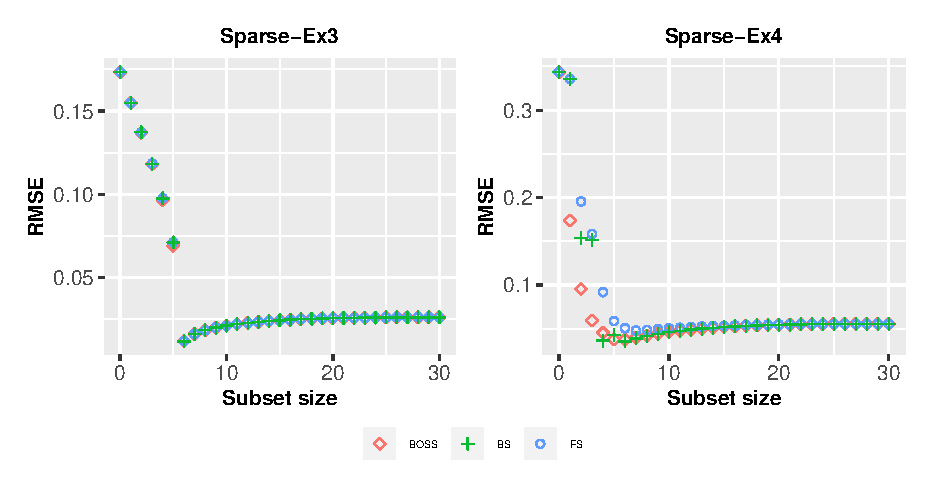
\includegraphics[width=\textwidth]{figures/rmse_solpath_lsmethods.eps}
	\caption{RMSE at each subset size, average over $1000$ replications. Note that for BOSS, the subset size $k_Q$ denotes the number of non-zero coefficients in $\tilde{\gamma}(k_Q)$. In both scenarios, we have $n=200$, $p=30$, $\rho=0.9$ and high SNR.}
	\label{fig:lossratio_fs_boss_k}
\end{figure}


\subsection{AICc-hdf as the selection rule for BOSS}

We apply AICc-hdf to choose the single optimal subset from the $K+1$ candidates. The implementation is discussed in step 6 of Algorithm \ref{alg:boss}. The hdf is calculated via Algorithm \ref{alg:hdf} based on the orthogonalized predictors $Q_{S_K}$. As to the estimation of $\mu$ and $\sigma$, if $n>p$, we use the OLS estimates based on the full model, i.e. $\hat{\mu}=Q_{S_{K}} z$, $\hat{\sigma}^2 = \lVert y-\hat{\mu} \rVert_2^2/(n-p)$. If $n \le p$, we use the estimates based on the lasso fit as discussed in \citet{reid2016study}, i.e. $\hat{\mu}=\hat{\mu}_l$ and $\hat{\sigma} = \sqrt{\lVert y-\hat{\mu}_l \rVert_2^2 / (n-\text{df}(\hat{\mu}_l)-1)}$, where $\hat{\mu}_l$ are the lasso fitted values based on 10-fold CV and df$(\hat{\mu}_l)$ is the corresponding number of non-zero coefficients in the lasso estimate. 

A numerical justification of using hdf is given in Figure \ref{fig:boss_aicc_hdf_kl}, where we compare averages of AICc-hdf and $\widehat{\text{Err}}_{\text{KL}}$ over $1000$ replications for BOSS under various true models. The sparse model (Sparse-Ex3) has $p_0=6$ predictors with non-zero coefficients, and all of the predictors in the dense model have non-zero coefficients ($p_0=p$). The correlation between predictors is $\rho=0.5$. We see that by using the sample average to represent the population mean, $E$(AICc-hdf) generally tracks the expected KL, $E(\text{Err}_{\text{KL}})$, reasonably well. Discrepancies can be observed at subset size $k<p_0$, where the set of true predictors is not entirely included in the model. The derivations of the classic AIC and AICc (both with ndf plugged in according to our notation) are based on an assumption that the true predictors are included in the model. In the situation where this assumption is violated, AICc will no longer be unbiased, and a similar conjecture can be made here for AICc in the context of BOSS. Last and most importantly, AICc-hdf yields the same average selected size as $\widehat{\text{Err}}_{\text{KL}}$ across all scenarios.

We find similar evidence in the Supplemental Material Figure \ref{fig:boss_cp_edf_hdf} that $E(\text{C}_p\text{-hdf})$ tracks the expected prediction error $E(\text{Err}_\text{SE})$ well in most cases, and they lead to the same average selected subset size; further supporting the use of hdf for BOSS. As discussed in Section \ref{sec:aicc_performance_bs}, using C$_p$ as the selection rule can perform poorly in practice because of the need to estimate $\sigma$. Evidence of a similar property when using C$_p$ as the selection rule for BOSS can be found in the Online Supplemental Material. For this reason, we prefer AICc in feasible versions of selection. 

% {fig:boss_aicc_hdf_kl}
\begin{figure}[ht!]
	\centering
	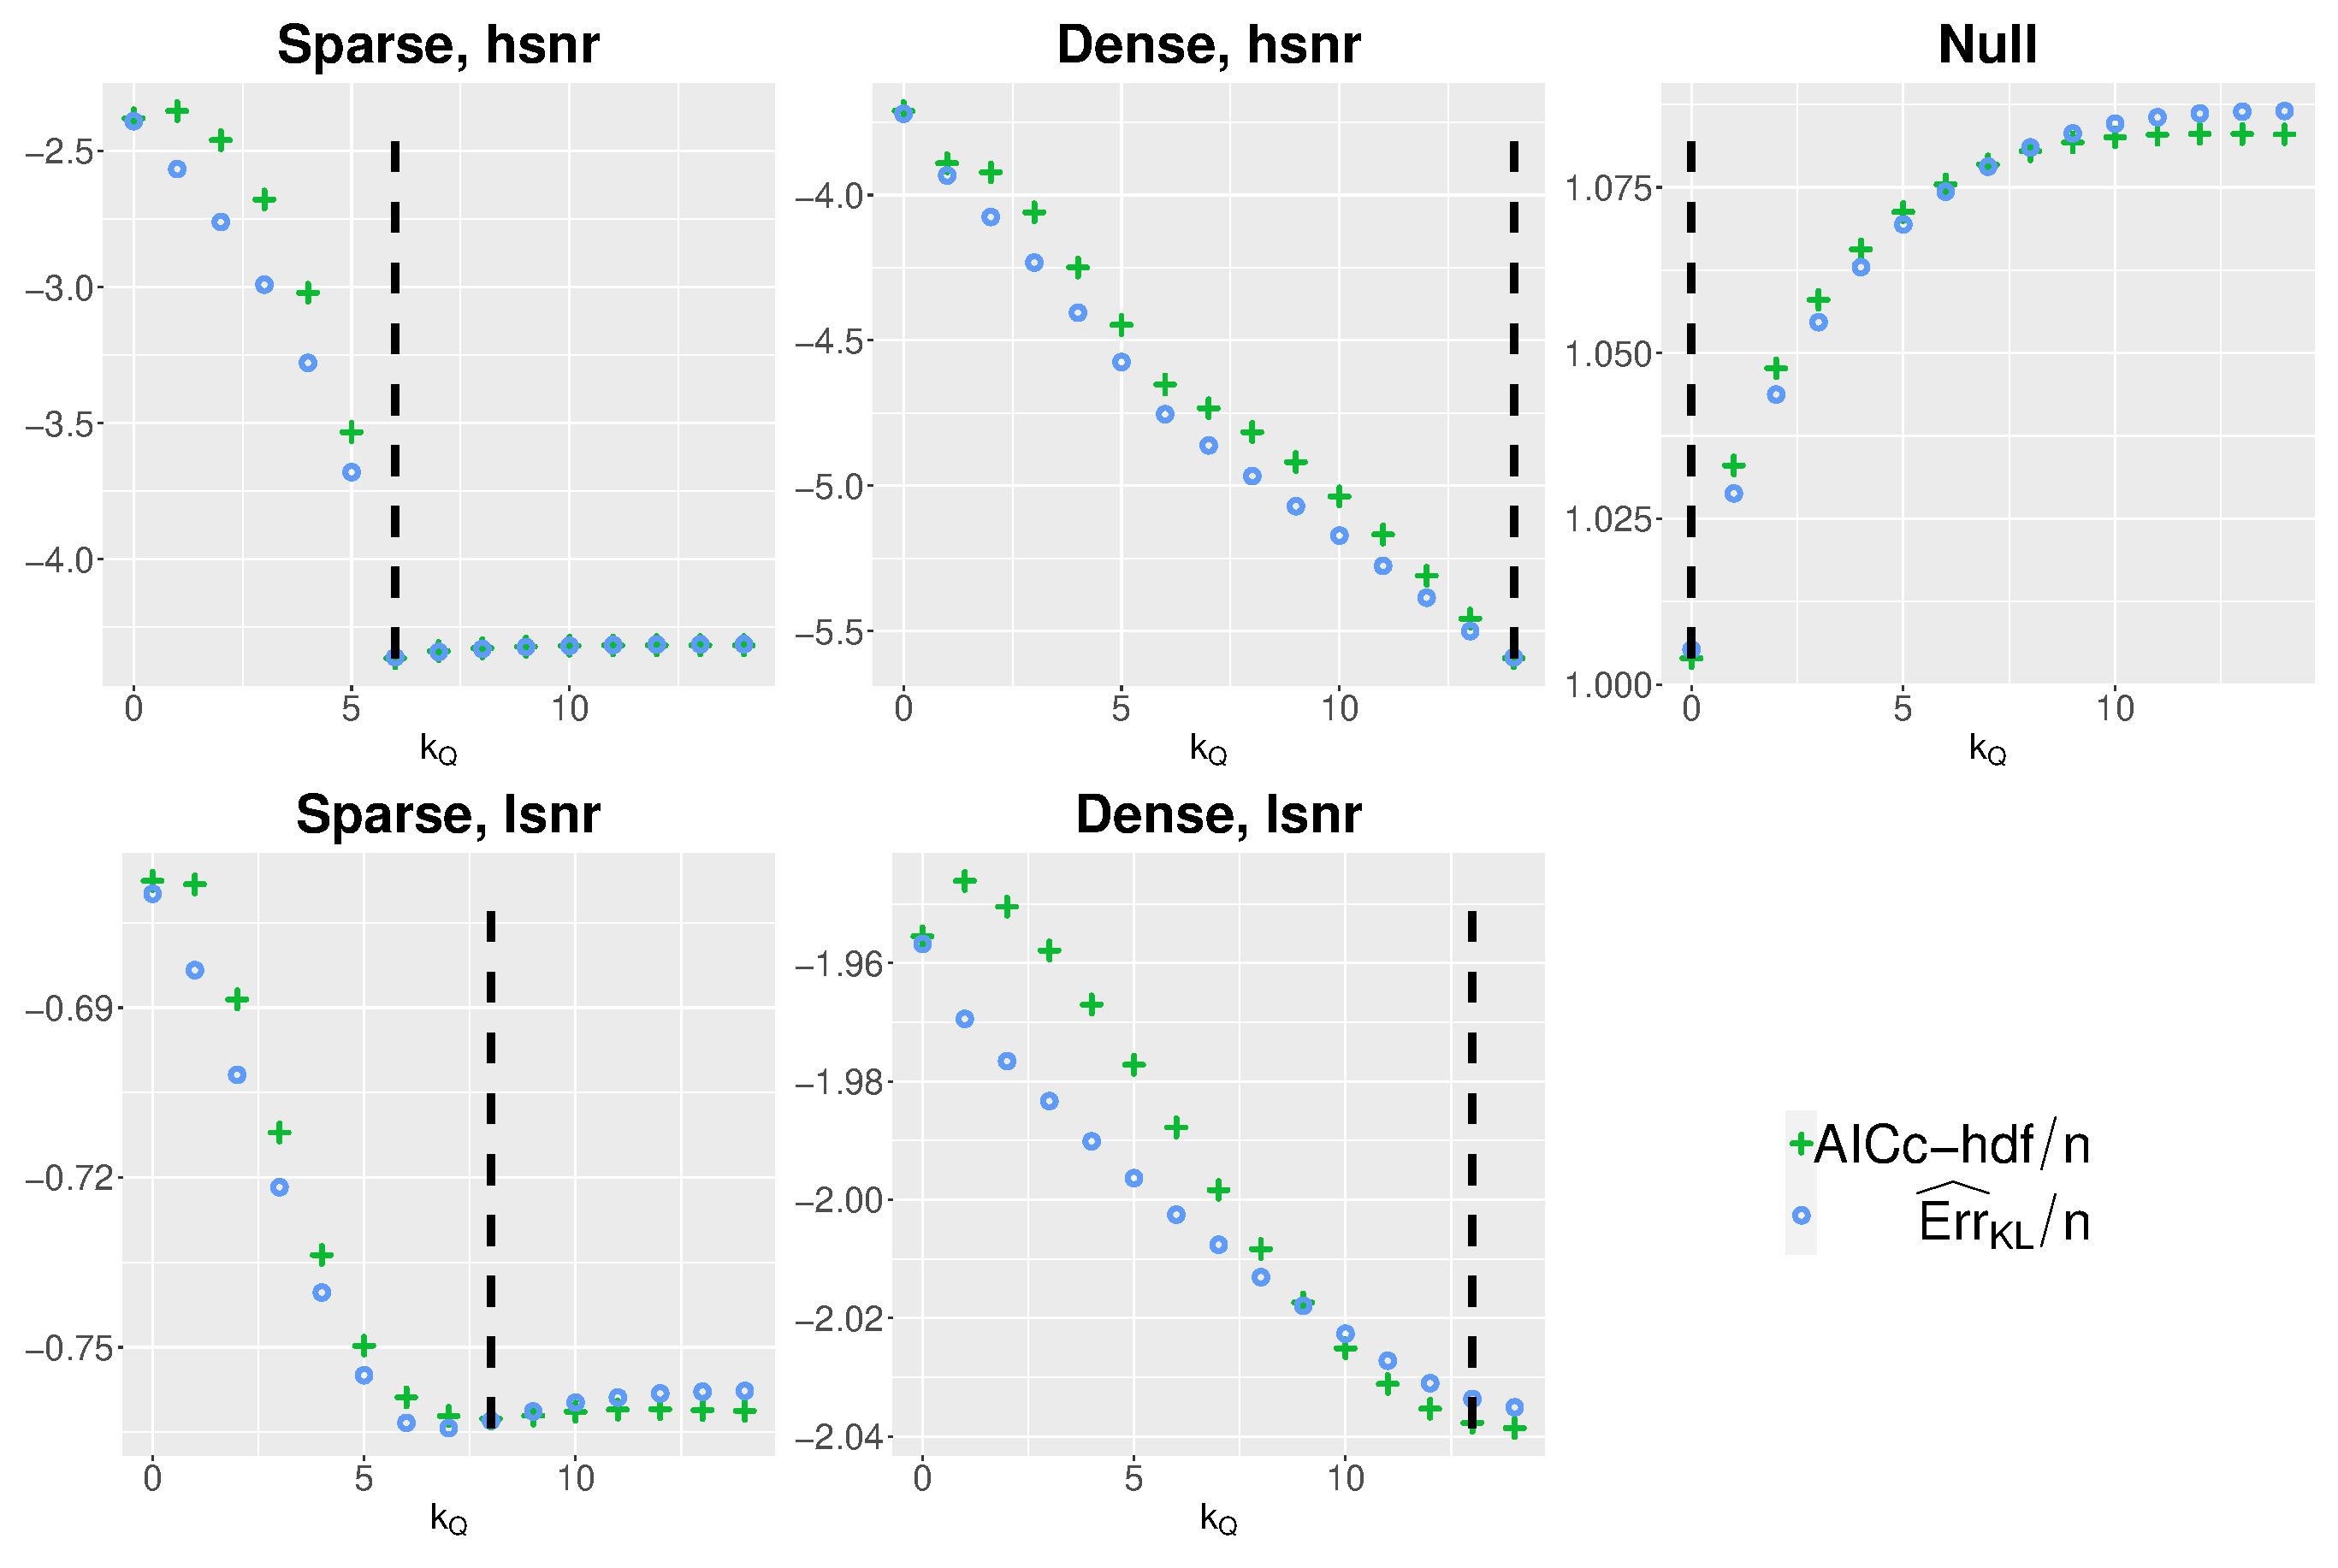
\includegraphics[width=0.9\textwidth]{figures/aicc_hdf_kl_boss.eps}
	\caption{Averages of AICc-hdf and $\widehat{\text{Err}}_{\text{KL}}$ for BOSS over $1000$ replications. Here $X$ is general with $n=200$, $p=14$. Both criteria result in the same average of the selected subset size over the $1000$ replications (rounded to the nearest integer) as denoted by the dashed vertical lines. }
	\label{fig:boss_aicc_hdf_kl}
\end{figure}


\subsection{The performance of BOSS in simulations}
\label{sec:boss_performance}
We now study the performance of BOSS via simulations. Besides the above mentioned Sparse-Ex3, Sparse-Ex4 and Dense designs, we consider two additional sparse model designs that have different correlation structures between predictors. For all of the sparse examples, we take $p_0=6$. We further consider three levels of the correlations, $\rho \in [0,0.5,0.9]$, and twelve combinations of $(n,p)$, resulting in a total of $540$ configuration options. For each configuration, $1000$ replications are constructed and we present similar evaluation measures as introduced in Section \ref{sec:aicc_performance_bs}. One measure is the $\%$ worse than the best possible BOSS, where the best possible BOSS means that on a single fit, we choose the subset size $k_Q$ with the minimum RMSE among all $K+1$ candidates, as if an oracle tells us the best model. The details of the simulation setup are discussed in the Supplemental Material Section \ref{sec:simulation_setup_generalx}. The full set of results can be found in the Online Supplemental Material.

We looked at results using AICc-hdf, C$_p$-hdf and 10-fold CV for BOSS, and AICc-hdf performed the best (see Online Supplemental Material), so results for that method are presented here. For FS, we studied several information criteria that have been proposed in the literature, e.g. EBIC \citep{wang2009forward}, HDBIC and HDHQ \citep{ing2011stepwise}. None of these criteria provide strong enough penalties for larger subset sizes. For high dimensional problems ($n<p$), they tend to choose subsets with size close to $n$, which is far from the truth for sparse designs ($p_0=6$). To remedy this overfitting problem, \citet{ing2011stepwise} suggests using a stopping rule, and one example is to only consider subsets with size $k < 5\sqrt{n / \log(p)}$. We find that this ad-hoc stopping rule avoids the problem of not penalizing larger subsets sufficiently, and provides reasonably good performance for sparse designs. However, for dense designs, using the stopping rule gives subsets that substantially underfit. It is clear that using a fixed stopping rule is not appropriate for all problems. For this reason, we prefer 10-fold CV as the selection rule for FS, and we find it overall outperforms these suggested information criteria (see Online Supplemental Material). Finally, we fit BS via the ``leaps'' algorithm for the case where $p \le 30$, and use 10-fold CV as the selection rule. BOSS and FS are fitted using our {\tt{R}} package \pkg{BOSSReg}\footnote{\url{https://github.com/sentian/BOSSreg}. A stable version of the R package is available on \textit{CRAN}.}, and the BS is fitted using the {\tt{R}} package \pkg{leaps} \citep{FortrancodebyAlanMiller2020}.

We also consider some popular regularization methods, including lasso \citep{Tibshirani1996}, SparseNet \citep{Mazumder2011} and gamma lasso \citep{Taddy2017}. We use the {\tt{R}} packages \pkg{glmnet} \citep{Friedman2010}, \pkg{sparsenet} \citep{Mazumder2011}, and \pkg{gamlr} \citep{Taddy2017}, respectively, to fit them, which are all available on \textit{CRAN}. We also consider a simplified version of the relaxed lasso \citep{Meinshausen2007}, which was discussed in \citet{Hastie2017} and can be fitted using the {\tt{R}} package \pkg{bestsubset}\footnote{The package is available at https://github.com/ryantibs/best-subset. We appreciate Prof. Ryan Tibshirani for the suggestion of fitting the simplified relaxed lasso.}. As to the selection rule, we use AICc for lasso, and 10-fold CV for the rest. In addition to these selectors, we have also considered 10-fold CV for lasso. We find (in the Online Supplement) that 10-fold CV performs similarly to AICc for lasso. In fact, the use of AICc for lasso was explored in \citet{Flynn2013}, where the authors proved that AICc is asymptotically efficient while performing similarly to CV. We further notice (results given in the Online Supplement) that SparseNet generally performs better than the relaxed lasso and gamma lasso, and hence only the results for SparseNet will be presented here. 

Note that there is an extensive list of regression estimators existing in the literature and the list is still growing fast. For instance, recent studies by \citet{hazimeh2020fast} and \citet{bertsimas2020sparse} considered regularized best subset problems that combine a lasso or ridge penalty with the cardinality constraint (either in the Lagrangian or constrained form), and the authors provided fast solvers by using modern optimization tools. We expect the general conclusions below regarding the relative performance of BOSS and regularization methods hold for the new methods. Our simulation code \footnote{The code is available at \url{https://github.com/sentian/BOSSreg}.} is structured to be easily extendable, and we invite interested readers to perform further comparisons.


A selected set of simulation results is presented in Table \ref{tab:boss_regu} and \ref{tab:boss_regu_highdim}. Here is a brief summary of the results:


\begin{itemize}
	\item For BOSS, AICc-hdf has a significant advantage over CV in terms of predictive performance, except for low SNR and $n$ is small, in which case the selection rules are comparable. CV is also ten times heavier in terms of computation than AICc-hdf. These results are similar to the comparison of AICc-hdf and CV for BS with an orthogonal $X$ as discussed in Section \ref{sec:aicc_performance_bs}. Overall, the simulations indicate that AICc with hdf used in place of edf is a reasonable selection rule for an LS-based method that can be applied in practice without the requirement that the predictors are orthogonal. In the following discussions, when we refer to BOSS, we mean BOSS-AICc-hdf. 

	\item The performance of BOSS is comparable to the performance of BS when BS is feasible. With a small sample size $n=200$, BOSS performs either similarly to or better than BS for a high SNR, and it performs either similarly to or slightly worse than BS for a low SNR. With a large sample size $n=2000$, BOSS is generally better than BS. Furthermore, BOSS only requires fitting the procedure once while BS uses CV as the selection rule, and a single fit of BOSS only has computational cost $O(npK)$ so that BOSS is feasible for high dimensional problems.

	\item The performance of BOSS is generally better than the performance of FS. In the Dense model, and Sparse-Ex3 with $n=200$ and low SNR, we see that BOSS performs similarly to FS. In all other scenarios, the advantage of BOSS is obvious. For example, in Sparse-Ex4 with $n=200$, high SNR and $\rho=0.9$, FS is almost ten times worse than BOSS in terms of RMSE. Recall that Sparse-Ex4 is an example where FS has trouble stepping in all of the true predictors (with $\beta_j \ne 0$) in early steps. This is evidenced by the fact that FS chooses eight extra predictors on average in this situation, while BOSS only chooses approximately two extra predictors. Furthermore, FS based on CV is ten times computationally heavier than BOSS. 

	\item Compared to the regularization methods, with a small sample size $n=200$, BOSS is the best when SNR is high, lasso is the best when SNR is low and SparseNet is in between. The lasso has the property of ``over-select and shrink,'' in order to retain less bias on the large non-zero estimates. In a high SNR, this property can result in disastrous performance, especially when $p$ is large. For example, in Sparse-Ex3, high SNR, $\rho=0.5$ and $p=180$, the relative efficiency of lasso is only $0.43$ and it significantly overfits. However, this property can be beneficial when SNR is low, as a method like BS has higher chance to miss the true predictors (less sparsistency). With a large sample size $n=550$ and $n=2000$, BOSS is almost always the best even when SNR is low. 

	\item In terms of support recovery in the sparse true models, LS-based methods can recover the true predictors (those with $\beta_j \ne 0$) and rarely include any noise predictors (those with $\beta_j = 0$) when SNR is high or the sample size $n$ is large. However, SparseNet and lasso generally overfit, with the latter being worse in that regard. In the low SNR and small $n$ scenario, lasso and SparseNet have more opportunity to recover the true predictors, but it comes with a price of including more false positives. 

\end{itemize}


Given the spirit of the summary above, it is important to point out the relevant work of \citet{Hastie2017}, where the authors provide a comprehensive set of simulation comparisons on BS, lasso and relaxed lasso. The authors concluded that BS performs the best in high SNR, lasso is the best in low SNR while relaxed lasso is in between. Given the similarity we have noticed between BOSS and BS, it is not surprising that this coincides with our results for BOSS here when sample size is relatively small ($n=200$). However, we find BOSS to be the best for large sample size $n$ even when the SNR is low (note that \citet{Hastie2017} did not examine any sample sizes greater than $n=500$). Moreover, it should be noted that \citet{Hastie2017} focus on the best possible performance of each method by applying a separate validation set drawn from the true model, rather than on feasible selection, as is considered in this study. 


% tab:boss_regu
% latex table generated in R 3.6.1 by xtable 1.8-4 package
% Sat Nov  9 17:57:42 2019
\begin{table}[ht]
\centering
\caption{The performance of BOSS compared to other methods for $n>p$. Selection rules are 'AICc-hdf/CV' for BOSS, 
                AICc for lasso and CV for the remaining methods in the table, respectively.} 
\label{tab:boss_regu}
\scalebox{0.5}{
\begin{tabular}{|c|c|c|c|ccccc|ccccc|ccccc|}
  \toprule 
 \multicolumn{1}{|r}{} & \multicolumn{1}{r}{} & \multicolumn{1}{r}{} &       & \multicolumn{5}{c|}{Sprse-Ex3}        & \multicolumn{5}{c|}{Sparse-Ex4}       & \multicolumn{5}{c|}{Dense} \\
 \cmidrule{5-19}\multicolumn{1}{|r}{} & \multicolumn{1}{r}{} & \multicolumn{1}{r}{} &       & BOSS  & BS    & FS    & lasso & SparseNet & BOSS  & BS    & FS    & lasso & SparseNet & BOSS  & BS    & FS    & lasso & \multicolumn{1}{c|}{SparseNet}  \\
 \cmidrule{5-19}\multicolumn{1}{|c}{} & \multicolumn{1}{c}{} & \multicolumn{1}{c}{} &       & \multicolumn{15}{c|}{\% worse than the best possible BOSS}  \\
 \midrule 
 \multirow{8}[4]{*}{n=200} & \multirow{4}[2]{*}{hsnr} & \multirow{2}[1]{*}{$\rho=0.5$} & p=30 & 2/22 & 24 & 22 & 70 & 14 & 19/24 & 23 & 28 & 49 & 21 & 1/8 & 9 & 8 & 2 & 5 \\ 
   &  &  & p=180 & 1/18 & - & 21 & 135 & 17 & 4/15 & - & 16 & 82 & 13 & 14/13 & - & 16 & 47 & 8 \\ 
   &  & \multirow{2}[1]{*}{$\rho=0.9$} & p=30 & 5/41 & 17 & 41 & 66 & 12 & 21/33 & 21 & 56 & 73 & 28 & 2/9 & 10 & 8 & 2 & 8 \\ 
   &  &  & p=180 & 3/27 & - & 29 & 126 & 16 & 7/34 & - & 68 & 123 & -10 & 15/12 & - & 12 & 71 & 20 \\ 
  \cmidrule{2-19} & \multirow{4}[2]{*}{lsnr} & \multirow{2}[1]{*}{$\rho=0.5$} & p=30 & 30/25 & 25 & 25 & 0 & 7 & 35/32 & 23 & 34 & 35 & 23 & 18/17 & 16 & 18 & 10 & 11 \\ 
   &  &  & p=180 & 11/13 & - & 13 & -3 & 3 & 31/26 & - & 34 & 33 & 20 & 4/8 & - & 9 & 2 & 6 \\ 
   &  & \multirow{2}[1]{*}{$\rho=0.9$} & p=30 & 28/24 & 23 & 23 & -2 & 5 & 32/27 & 18 & 78 & 71 & 44 & 15/14 & 15 & 13 & 10 & 12 \\ 
   &  &  & p=180 & 16/16 & - & 15 & -5 & 1 & 17/18 & - & 36 & 33 & 35 & 12/10 & - & 10 & 15 & 9 \\ 
  \midrule \multirow{8}[4]{*}{n=2000} & \multirow{4}[2]{*}{hsnr} & \multirow{2}[1]{*}{$\rho=0.5$} & p=30 & 3/22 & 22 & 21 & 73 & 14 & 7/29 & 21 & 23 & 86 & 12 & 0/3 & 0 & 0 & 1 & 0 \\ 
   &  &  & p=180 & 1/22 & - & 22 & 130 & 14 & 6/28 & - & 21 & 174 & 12 & 8/9 & - & 12 & 37 & 8 \\ 
   &  & \multirow{2}[1]{*}{$\rho=0.9$} & p=30 & 2/21 & 21 & 22 & 74 & 13 & 32/33 & 16 & 33 & 108 & 12 & 0/3 & 1 & 1 & 2 & 1 \\ 
   &  &  & p=180 & 1/21 & - & 22 & 135 & 14 & 15/25 & - & 90 & 226 & 10 & 10/10 & - & 9 & 39 & 17 \\ 
  \cmidrule{2-19} & \multirow{4}[2]{*}{lsnr} & \multirow{2}[1]{*}{$\rho=0.5$} & p=30 & 5/22 & 21 & 21 & 73 & 14 & 13/30 & 22 & 23 & 61 & 15 & 2/9 & 10 & 10 & 2 & 7 \\ 
   &  &  & p=180 & 5/22 & - & 22 & 129 & 13 & 8/27 & - & 20 & 125 & 10 & 11/13 & - & 16 & 32 & 10 \\ 
   &  & \multirow{2}[1]{*}{$\rho=0.9$} & p=30 & 5/21 & 20 & 21 & 53 & 3 & 27/34 & 16 & 40 & 85 & 12 & 3/11 & 11 & 9 & 3 & 8 \\ 
   &  &  & p=180 & 4/17 & - & 17 & 92 & -5 & 14/27 & - & 104 & 179 & 20 & 12/13 & - & 11 & 40 & 18 \\ 
   \midrule 
 \multicolumn{1}{|c}{} & \multicolumn{1}{c}{} & \multicolumn{1}{c}{} &       & \multicolumn{15}{c|}{Relative efficiency} \\
 \midrule 
\multirow{8}[4]{*}{n=200} & \multirow{4}[2]{*}{hsnr} & \multirow{2}[1]{*}{$\rho=0.5$} & p=30 & 1/0.84 & 0.82 & 0.84 & 0.6 & 0.9 & 1/0.96 & 0.97 & 0.93 & 0.8 & 0.99 & 0.98/0.93 & 0.91 & 0.93 & 0.98 & 0.94 \\ 
   &  &  & p=180 & 1/0.85 & - & 0.84 & 0.43 & 0.86 & 1/0.91 & - & 0.9 & 0.57 & 0.92 & 0.95/0.96 & - & 0.93 & 0.73 & 1 \\ 
   &  & \multirow{2}[1]{*}{$\rho=0.9$} & p=30 & 1/0.74 & 0.9 & 0.74 & 0.63 & 0.93 & 1/0.91 & 1 & 0.78 & 0.7 & 0.95 & 0.98/0.91 & 0.9 & 0.92 & 0.98 & 0.93 \\ 
   &  &  & p=180 & 1/0.8 & - & 0.79 & 0.45 & 0.88 & 0.84/0.68 & - & 0.54 & 0.41 & 1 & 0.97/1 & - & 1 & 0.65 & 0.93 \\ 
  \cmidrule{2-19} & \multirow{4}[2]{*}{lsnr} & \multirow{2}[1]{*}{$\rho=0.5$} & p=30 & 0.77/0.8 & 0.8 & 0.8 & 1 & 0.93 & 0.91/0.93 & 1 & 0.92 & 0.91 & 1 & 0.93/0.94 & 0.95 & 0.93 & 1 & 0.99 \\ 
   &  &  & p=180 & 0.87/0.86 & - & 0.86 & 1 & 0.94 & 0.92/0.96 & - & 0.9 & 0.91 & 1 & 0.97/0.94 & - & 0.94 & 1 & 0.96 \\ 
   &  & \multirow{2}[1]{*}{$\rho=0.9$} & p=30 & 0.76/0.79 & 0.8 & 0.8 & 1 & 0.93 & 0.89/0.93 & 1 & 0.66 & 0.69 & 0.82 & 0.96/0.97 & 0.96 & 0.97 & 1 & 0.98 \\ 
   &  &  & p=180 & 0.82/0.82 & - & 0.83 & 1 & 0.95 & 1/0.99 & - & 0.86 & 0.88 & 0.87 & 0.97/0.99 & - & 1 & 0.95 & 1 \\ 
  \midrule \multirow{8}[4]{*}{n=2000} & \multirow{4}[2]{*}{hsnr} & \multirow{2}[1]{*}{$\rho=0.5$} & p=30 & 1/0.85 & 0.85 & 0.85 & 0.59 & 0.91 & 1/0.83 & 0.89 & 0.87 & 0.58 & 0.96 & 0.98/0.96 & 0.98 & 0.98 & 0.97 & 0.98 \\ 
   &  &  & p=180 & 1/0.83 & - & 0.83 & 0.44 & 0.89 & 1/0.83 & - & 0.88 & 0.39 & 0.95 & 1/0.99 & - & 0.96 & 0.79 & 1 \\ 
   &  & \multirow{2}[1]{*}{$\rho=0.9$} & p=30 & 1/0.84 & 0.85 & 0.84 & 0.59 & 0.9 & 0.84/0.84 & 0.96 & 0.84 & 0.54 & 1 & 1/0.97 & 0.99 & 0.99 & 0.98 & 0.99 \\ 
   &  &  & p=180 & 1/0.84 & - & 0.83 & 0.43 & 0.89 & 0.96/0.88 & - & 0.58 & 0.34 & 1 & 0.99/0.99 & - & 1 & 0.78 & 0.93 \\ 
  \cmidrule{2-19} & \multirow{4}[2]{*}{lsnr} & \multirow{2}[1]{*}{$\rho=0.5$} & p=30 & 1/0.86 & 0.86 & 0.86 & 0.61 & 0.92 & 1/0.87 & 0.93 & 0.92 & 0.7 & 0.99 & 0.98/0.91 & 0.9 & 0.91 & 0.98 & 0.93 \\ 
   &  &  & p=180 & 1/0.86 & - & 0.86 & 0.46 & 0.93 & 1/0.85 & - & 0.9 & 0.48 & 0.98 & 1/0.97 & - & 0.95 & 0.83 & 1 \\ 
   &  & \multirow{2}[1]{*}{$\rho=0.9$} & p=30 & 0.98/0.85 & 0.86 & 0.85 & 0.67 & 1 & 0.88/0.83 & 0.97 & 0.8 & 0.61 & 1 & 1/0.92 & 0.92 & 0.94 & 1 & 0.95 \\ 
   &  &  & p=180 & 0.91/0.81 & - & 0.81 & 0.49 & 1 & 1/0.9 & - & 0.56 & 0.41 & 0.95 & 0.99/0.99 & - & 1 & 0.8 & 0.94 \\ 
   \midrule 
 \multicolumn{1}{|c}{} & \multicolumn{1}{c}{} & \multicolumn{1}{c}{} &       & \multicolumn{15}{c|}{Sparsistency (number of extra variables)} \\
 \midrule 
\multirow{8}[4]{*}{n=200} & \multirow{4}[2]{*}{hsnr} & \multirow{2}[1]{*}{$\rho=0.5$} & p=30 & 6(0)/6(0.6) & 6(0.7) & 6(0.6) & 6(7.9) & 6(1.1) & 4.4(0.2)/5(1) & 5(1) & 4.8(1.1) & 5.7(10.4) & 4.8(2.1) & 29.6/26.1 & 25.1 & 26 & 29.1 & 27 \\ 
   &  &  & p=180 & 6(0)/6(0.3) & - & 6(0.4) & 6(16.6) & 6(2.4) & 4(0)/4.2(0.5) & - & 4.1(0.5) & 5.1(20.2) & 4.2(3.5) & 17/20.2 & - & 19.6 & 52.2 & 32.4 \\ 
   &  & \multirow{2}[1]{*}{$\rho=0.9$} & p=30 & 6(0.6)/6(2.1) & 6(0.8) & 6(2.1) & 6(9.2) & 6(1.6) & 5.1(2.8)/5.3(3.8) & 5(1) & 4.8(4.1) & 5.8(17.8) & 4.4(2.7) & 29.3/25.2 & 23 & 24.6 & 28.9 & 26.2 \\ 
   &  &  & p=180 & 6(0.1)/6(0.6) & - & 6(0.6) & 6(16.2) & 6(2.4) & 4.2(2.4)/4.3(4.3) & - & 4.3(8) & 4.6(44.2) & 4.1(3.1) & 15.6/21.3 & - & 17.2 & 54.4 & 37.7 \\ 
  \cmidrule{2-19} & \multirow{4}[2]{*}{lsnr} & \multirow{2}[1]{*}{$\rho=0.5$} & p=30 & 2.9(2)/3.6(2.4) & 3.4(2.1) & 3.5(2.3) & 5.1(6.9) & 4.7(5.3) & 2.3(1)/2.7(1.3) & 2.6(1) & 2.6(1.5) & 3.6(6.9) & 2.8(2.9) & 5.7/7.5 & 6.6 & 7.1 & 5.3 & 10.3 \\ 
   &  &  & p=180 & 0.3(0.1)/1(0.7) & - & 1(0.7) & 3(9.7) & 2.6(9.3) & 1(0.2)/1.6(0.9) & - & 1.3(0.8) & 2.2(10.7) & 2.1(6.5) & 0.2/1.1 & - & 0.9 & 2.7 & 6.9 \\ 
   &  & \multirow{2}[1]{*}{$\rho=0.9$} & p=30 & 1.9(2.3)/2.4(3) & 2.5(2.8) & 2.4(2.9) & 3.9(7.5) & 3.7(6.1) & 2.7(3.9)/3.2(5) & 2.7(0.9) & 2.2(4.4) & 3(10.1) & 2.9(8) & 4.1/5.2 & 4.3 & 4.5 & 8.4 & 5.9 \\ 
   &  &  & p=180 & 0.5(0.2)/1.1(1.1) & - & 1.1(1.1) & 3.2(11.1) & 3(10.8) & 0.7(1.7)/1.1(5.5) & - & 0.2(0.6) & 0.3(4.8) & 0.6(9) & 1/2.1 & - & 1.6 & 3.9 & 3.3 \\ 
  \midrule \multirow{8}[4]{*}{n=2000} & \multirow{4}[2]{*}{hsnr} & \multirow{2}[1]{*}{$\rho=0.5$} & p=30 & 6(0.1)/6(0.6) & 6(0.6) & 6(0.6) & 6(8.4) & 6(1) & 6(0.2)/6(0.6) & 6(0.6) & 6(0.6) & 6(10.9) & 6(0.8) & 30/30 & 30 & 30 & 30 & 30 \\ 
   &  &  & p=180 & 6(0)/6(0.4) & - & 6(0.4) & 6(21.5) & 6(2.3) & 6(0.1)/6(0.3) & - & 6(0.3) & 6(32.2) & 6(1.3) & 34.5/35.1 & - & 32.6 & 106.5 & 43 \\ 
   &  & \multirow{2}[1]{*}{$\rho=0.9$} & p=30 & 6(0)/6(0.6) & 6(0.6) & 6(0.6) & 6(9.2) & 6(1) & 6(0.4)/6(0.7) & 6(0.6) & 6(1.3) & 6(17.8) & 6(1.6) & 30/29.9 & 29.9 & 29.9 & 30 & 30 \\ 
   &  &  & p=180 & 6(0)/6(0.4) & - & 6(0.4) & 6(23.2) & 6(2.2) & 6(1.4)/6(1.7) & - & 5.9(3.8) & 6(72.7) & 6(8.7) & 35/38.6 & - & 30.2 & 109.6 & 52.4 \\ 
  \cmidrule{2-19} & \multirow{4}[2]{*}{lsnr} & \multirow{2}[1]{*}{$\rho=0.5$} & p=30 & 6(0.1)/6(0.6) & 6(0.6) & 6(0.6) & 6(8.3) & 6(0.7) & 4.2(0.4)/4.3(0.7) & 4.3(0.6) & 4.2(0.7) & 5.2(9.6) & 4.3(1) & 29/22.7 & 21.2 & 22.1 & 28 & 24.1 \\ 
   &  &  & p=180 & 6(0.1)/6(0.4) & - & 6(0.4) & 6(21.2) & 6(0.9) & 4(0.1)/4(0.4) & - & 4(0.4) & 4.6(26.1) & 4.1(1.3) & 16/17 & - & 14.3 & 61.8 & 25.3 \\ 
   &  & \multirow{2}[1]{*}{$\rho=0.9$} & p=30 & 5.8(0.3)/5.8(1.1) & 5.8(1.1) & 5.8(1.1) & 6(9.2) & 6(0.8) & 4.4(1.9)/4.4(1.7) & 4.3(0.6) & 4.3(2.2) & 5.4(16.6) & 4.2(2.5) & 28.8/21.2 & 18.5 & 20.2 & 27.6 & 23.5 \\ 
   &  &  & p=180 & 5.7(0.3)/5.7(0.7) & - & 5.7(0.7) & 6(23) & 6(1) & 4.1(3.6)/4.1(4.4) & - & 3.7(3.7) & 4.6(60.3) & 4.2(14.2) & 16.6/21.4 & - & 11.8 & 65.3 & 32.3 \\ 
   \bottomrule 
\end{tabular}
}
\end{table}

% tab:boss_regu_highdim
% latex table generated in R 3.6.2 by xtable 1.8-4 package
% Thu Feb 13 10:46:28 2020
\begin{table}[ht]
\centering
\caption{The performance of BOSS compared to other methods for $n \le p$. Selection rules are for 'AICc-hdf/CV' for BOSS, 
                AICc for lasso and CV for the remaining methods in the table, respectively.} 
\label{tab:boss_regu_highdim}
\scalebox{0.52}{
\begin{tabular}{|c|c|c|c|ccccc|ccccc|ccccc|}
  \toprule 
 \multicolumn{1}{|r}{} & \multicolumn{1}{r}{} & \multicolumn{1}{r}{} &       & \multicolumn{5}{c|}{Sprse-Ex3}        & \multicolumn{5}{c|}{Sparse-Ex4}       & \multicolumn{5}{c|}{Dense} \\
 \cmidrule{5-19}\multicolumn{1}{|r}{} & \multicolumn{1}{r}{} & \multicolumn{1}{r}{} &       & BOSS  & BS & FS    & lasso    & SparseNet & BOSS  & BS & FS    & lasso    & SparseNet & BOSS  & BS & FS    & lasso  & \multicolumn{1}{c|}{SparseNet}  \\
 \cmidrule{5-19}\multicolumn{1}{|c}{} & \multicolumn{1}{c}{} & \multicolumn{1}{c}{} &       & \multicolumn{15}{c|}{\% worse than the best possible BOSS}  \\
 \midrule 
 \multirow{8}[4]{*}{n=200} & \multirow{4}[2]{*}{hsnr} & \multirow{2}[1]{*}{$\rho=0.5$} & p=550 & 2/19 & - & 20 & 168 & 25 & 4/10 & - & 11 & 94 & 12 & 7/13 & - & 13 & 70 & 3 \\ 
   &  &  & p=1000 & 9/18 & - & 18 & 176 & 25 & 8/10 & - & 11 & 103 & 13 & 7/15 & - & 17 & 113 & 3 \\ 
   &  & \multirow{2}[1]{*}{$\rho=0.9$} & p=550 & 6/48 & - & 48 & 150 & 38 & 9/33 & - & 67 & 186 & -9 & 14/14 & - & 17 & 131 & 17 \\ 
   &  &  & p=1000 & 14/37 & - & 38 & 167 & 22 & 16/99 & - & 122 & 198 & -21 & 11/14 & - & 18 & 158 & 125 \\ 
  \cmidrule{2-19} & \multirow{4}[2]{*}{lsnr} & \multirow{2}[1]{*}{$\rho=0.5$} & p=550 & 10/9 & - & 9 & -4 & 3 & 23/21 & - & 28 & 27 & 20 & 5/6 & - & 6 & 1 & 4 \\ 
   &  &  & p=1000 & 15/10 & - & 10 & -2 & 4 & 19/15 & - & 19 & 15 & 15 & 6/6 & - & 6 & 0 & 4 \\ 
   &  & \multirow{2}[1]{*}{$\rho=0.9$} & p=550 & 10/10 & - & 10 & -4 & 2 & 6/8 & - & 11 & 9 & 11 & 18/13 & - & 12 & 13 & 11 \\ 
   &  &  & p=1000 & 15/8 & - & 8 & -4 & 2 & 5/5 & - & 7 & 3 & 6 & 15/12 & - & 12 & 12 & 9 \\ 
  \midrule \multirow{8}[4]{*}{n=500} & \multirow{4}[2]{*}{hsnr} & \multirow{2}[1]{*}{$\rho=0.5$} & p=550 & 0/20 & - & 22 & 157 & 19 & 31/26 & - & 37 & 97 & 30 & 9/10 & - & 13 & 57 & 8 \\ 
   &  &  & p=1000 & 1/21 & - & 22 & 172 & 21 & 29/25 & - & 36 & 114 & 29 & 8/11 & - & 14 & 85 & 9 \\ 
   &  & \multirow{2}[1]{*}{$\rho=0.9$} & p=550 & 1/22 & - & 23 & 158 & 19 & 12/18 & - & 30 & 162 & 29 & 13/10 & - & 14 & 79 & 23 \\ 
   &  &  & p=1000 & 2/22 & - & 23 & 175 & 21 & 8/13 & - & 21 & 172 & 19 & 12/11 & - & 14 & 107 & 33 \\ 
  \cmidrule{2-19} & \multirow{4}[2]{*}{lsnr} & \multirow{2}[1]{*}{$\rho=0.5$} & p=550 & 34/28 & - & 28 & 23 & 21 & 24/31 & - & 33 & 71 & 28 & 16/12 & - & 14 & 17 & 11 \\ 
   &  &  & p=1000 & 25/26 & - & 26 & 21 & 18 & 17/25 & - & 26 & 67 & 20 & 14/12 & - & 15 & 17 & 11 \\ 
   &  & \multirow{2}[1]{*}{$\rho=0.9$} & p=550 & 30/25 & - & 26 & 18 & 17 & 12/14 & - & 73 & 82 & 34 & 6/7 & - & 8 & 14 & 10 \\ 
   &  &  & p=1000 & 25/26 & - & 25 & 17 & 15 & 6/10 & - & 41 & 44 & 28 & 7/7 & - & 8 & 17 & 12 \\ 
   \midrule 
 \multicolumn{1}{|c}{} & \multicolumn{1}{c}{} & \multicolumn{1}{c}{} &       & \multicolumn{15}{c|}{Relative efficiency} \\
 \midrule 
\multirow{8}[4]{*}{n=200} & \multirow{4}[2]{*}{hsnr} & \multirow{2}[1]{*}{$\rho=0.5$} & p=550 & 1/0.85 & - & 0.84 & 0.38 & 0.81 & 1/0.95 & - & 0.93 & 0.54 & 0.92 & 0.96/0.91 & - & 0.91 & 0.6 & 1 \\ 
   &  &  & p=1000 & 1/0.92 & - & 0.92 & 0.39 & 0.87 & 1/0.99 & - & 0.98 & 0.53 & 0.96 & 0.96/0.9 & - & 0.88 & 0.48 & 1 \\ 
   &  & \multirow{2}[1]{*}{$\rho=0.9$} & p=550 & 1/0.72 & - & 0.72 & 0.43 & 0.77 & 0.84/0.68 & - & 0.55 & 0.32 & 1 & 1/1 & - & 0.98 & 0.49 & 0.97 \\ 
   &  &  & p=1000 & 1/0.83 & - & 0.82 & 0.43 & 0.93 & 0.68/0.4 & - & 0.36 & 0.27 & 1 & 1/0.97 & - & 0.94 & 0.43 & 0.49 \\ 
  \cmidrule{2-19} & \multirow{4}[2]{*}{lsnr} & \multirow{2}[1]{*}{$\rho=0.5$} & p=550 & 0.88/0.88 & - & 0.88 & 1 & 0.94 & 0.97/0.99 & - & 0.94 & 0.94 & 1 & 0.96/0.95 & - & 0.95 & 1 & 0.97 \\ 
   &  &  & p=1000 & 0.85/0.89 & - & 0.89 & 1 & 0.94 & 0.96/1 & - & 0.96 & 1 & 1 & 0.95/0.95 & - & 0.95 & 1 & 0.97 \\ 
   &  & \multirow{2}[1]{*}{$\rho=0.9$} & p=550 & 0.87/0.87 & - & 0.87 & 1 & 0.94 & 1/0.98 & - & 0.95 & 0.97 & 0.95 & 0.95/0.99 & - & 0.99 & 0.98 & 1 \\ 
   &  &  & p=1000 & 0.84/0.89 & - & 0.89 & 1 & 0.94 & 0.98/0.98 & - & 0.97 & 1 & 0.98 & 0.94/0.98 & - & 0.98 & 0.98 & 1 \\ 
  \midrule \multirow{8}[4]{*}{n=500} & \multirow{4}[2]{*}{hsnr} & \multirow{2}[1]{*}{$\rho=0.5$} & p=550 & 1/0.84 & - & 0.83 & 0.39 & 0.85 & 0.96/1 & - & 0.92 & 0.64 & 0.97 & 0.99/0.98 & - & 0.95 & 0.69 & 1 \\ 
   &  &  & p=1000 & 1/0.84 & - & 0.83 & 0.37 & 0.84 & 0.97/1 & - & 0.91 & 0.58 & 0.97 & 1/0.97 & - & 0.94 & 0.58 & 0.99 \\ 
   &  & \multirow{2}[1]{*}{$\rho=0.9$} & p=550 & 1/0.82 & - & 0.82 & 0.39 & 0.84 & 1/0.95 & - & 0.87 & 0.43 & 0.87 & 0.98/1 & - & 0.97 & 0.62 & 0.89 \\ 
   &  &  & p=1000 & 1/0.83 & - & 0.82 & 0.37 & 0.84 & 1/0.95 & - & 0.89 & 0.4 & 0.91 & 0.99/1 & - & 0.97 & 0.54 & 0.84 \\ 
  \cmidrule{2-19} & \multirow{4}[2]{*}{lsnr} & \multirow{2}[1]{*}{$\rho=0.5$} & p=550 & 0.9/0.94 & - & 0.95 & 0.98 & 1 & 1/0.95 & - & 0.93 & 0.73 & 0.97 & 0.96/0.99 & - & 0.97 & 0.95 & 1 \\ 
   &  &  & p=1000 & 0.94/0.93 & - & 0.93 & 0.97 & 1 & 1/0.94 & - & 0.93 & 0.7 & 0.97 & 0.98/0.99 & - & 0.97 & 0.95 & 1 \\ 
   &  & \multirow{2}[1]{*}{$\rho=0.9$} & p=550 & 0.9/0.93 & - & 0.93 & 0.99 & 1 & 1/0.98 & - & 0.65 & 0.61 & 0.84 & 1/0.99 & - & 0.98 & 0.93 & 0.97 \\ 
   &  &  & p=1000 & 0.92/0.92 & - & 0.92 & 0.98 & 1 & 1/0.97 & - & 0.76 & 0.74 & 0.83 & 1/1 & - & 1 & 0.91 & 0.96 \\ 
   \midrule 
 \multicolumn{1}{|c}{} & \multicolumn{1}{c}{} & \multicolumn{1}{c}{} &       & \multicolumn{15}{c|}{Sparsistency (number of extra variables)} \\
 \midrule 
\multirow{8}[4]{*}{n=200} & \multirow{4}[2]{*}{hsnr} & \multirow{2}[1]{*}{$\rho=0.5$} & p=550 & 6(0)/6(0.3) & - & 6(0.3) & 6(19.7) & 6(4.1) & 4(0.1)/4.1(0.3) & - & 4.1(0.3) & 4.7(23.2) & 4.3(5.3) & 16.5/15.9 & - & 15.7 & 52.8 & 29.4 \\ 
   &  &  & p=1000 & 6(0.3)/6(0.2) & - & 6(0.2) & 6(20.4) & 6(4.6) & 4.1(0.5)/4.1(0.3) & - & 4.1(0.3) & 4.4(24.3) & 4.2(5.4) & 17.9/15 & - & 14.6 & 45.9 & 34.5 \\ 
   &  & \multirow{2}[1]{*}{$\rho=0.9$} & p=550 & 6(0.6)/6(1.4) & - & 6(1.3) & 6(20.5) & 6(9.3) & 4(2)/4(2.9) & - & 4(7.1) & 4.1(61.2) & 4.1(4.7) & 13.3/15.6 & - & 13.1 & 32.8 & 45.1 \\ 
   &  &  & p=1000 & 6(0.6)/6(0.8) & - & 6(0.8) & 6(20.8) & 6(5.3) & 3.8(6.3)/3.8(5.7) & - & 3.5(10.5) & 4(67) & 4(6.6) & 14.6/17.2 & - & 16.2 & 7.6 & 22.3 \\ 
  \cmidrule{2-19} & \multirow{4}[2]{*}{lsnr} & \multirow{2}[1]{*}{$\rho=0.5$} & p=550 & 0.4(0.3)/0.7(0.4) & - & 0.7(0.4) & 2.6(11.6) & 2.4(13.8) & 0.9(0.4)/1.1(0.7) & - & 0.8(0.6) & 1.5(11.6) & 1.6(10.1) & 0.2/0.6 & - & 0.6 & 8.3 & 8.3 \\ 
   &  &  & p=1000 & 0.6(1.1)/0.5(0.4) & - & 0.6(0.4) & 2.2(10.9) & 2.1(14.2) & 0.8(1.2)/0.6(0.5) & - & 0.4(0.4) & 1(9.3) & 1.2(10.7) & 0.5/0.5 & - & 0.5 & 8 & 8.4 \\ 
   &  & \multirow{2}[1]{*}{$\rho=0.9$} & p=550 & 0.4(0.5)/0.5(0.7) & - & 0.5(0.7) & 2.1(12.3) & 2.1(14.5) & 0.3(0.4)/0.3(0.6) & - & 0.1(0.3) & 0.2(6.7) & 0.2(7.7) & 0.8/1.5 & - & 1.4 & 7.8 & 4.2 \\ 
   &  &  & p=1000 & 0.5(1.5)/0.4(0.4) & - & 0.4(0.4) & 2(11.3) & 1.9(15.3) & 0.1(0.5)/0.1(0.4) & - & 0(0.3) & 0.1(6.3) & 0.1(6.6) & 0.8/1.2 & - & 1.2 & 9 & 5.1 \\ 
  \midrule \multirow{8}[4]{*}{n=500} & \multirow{4}[2]{*}{hsnr} & \multirow{2}[1]{*}{$\rho=0.5$} & p=550 & 6(0)/6(0.3) & - & 6(0.3) & 6(24.1) & 6(3.4) & 4.6(0.1)/5.1(0.8) & - & 4.8(0.6) & 5.7(31.8) & 5.1(6.5) & 21.8/23.1 & - & 21.3 & 109.5 & 34.3 \\ 
   &  &  & p=1000 & 6(0)/6(0.3) & - & 6(0.3) & 6(26.6) & 6(4.1) & 4.7(0.2)/5.1(0.8) & - & 4.7(0.5) & 5.4(37.2) & 5(7.1) & 22.2/21.8 & - & 20.4 & 99.8 & 35.7 \\ 
   &  & \multirow{2}[1]{*}{$\rho=0.9$} & p=550 & 6(0)/6(0.3) & - & 6(0.3) & 6(24.5) & 6(3.4) & 4.4(1.6)/4.5(4) & - & 4.1(0.4) & 4.7(66.3) & 4.1(4.2) & 20.8/27 & - & 19.8 & 131.9 & 55.4 \\ 
   &  &  & p=1000 & 6(0)/6(0.3) & - & 6(0.3) & 6(27.6) & 6(4) & 4.3(0.9)/4.3(1.9) & - & 4(0.4) & 4.4(81.5) & 4.1(4.7) & 19.6/22.3 & - & 17.7 & 147.5 & 61.2 \\ 
  \cmidrule{2-19} & \multirow{4}[2]{*}{lsnr} & \multirow{2}[1]{*}{$\rho=0.5$} & p=550 & 3.5(0.3)/4.1(1) & - & 4.1(0.9) & 5.8(23.4) & 5.2(12.1) & 2.7(0.3)/2.9(0.6) & - & 2.7(0.6) & 3.7(24.2) & 2.9(4.6) & 2.1/4.2 & - & 2.9 & 22.4 & 13 \\ 
   &  &  & p=1000 & 3.6(0.5)/3.8(0.9) & - & 3.8(0.9) & 5.6(25.1) & 4.9(13.6) & 2.5(0.4)/2.5(0.6) & - & 2.3(0.5) & 3.1(26.3) & 2.6(4.8) & 2.2/3.7 & - & 2.5 & 19.2 & 13.2 \\ 
   &  & \multirow{2}[1]{*}{$\rho=0.9$} & p=550 & 3(0.9)/3.5(1.7) & - & 3.5(1.7) & 5.3(23.7) & 4.6(13.5) & 2.3(10.3)/2.5(13.9) & - & 0.8(1.2) & 1.3(21.2) & 2.2(34.3) & 1.5/3.9 & - & 2 & 10.4 & 4 \\ 
   &  &  & p=1000 & 3(1.1)/3.1(1.4) & - & 3.1(1.4) & 5.1(25.9) & 4.4(15) & 1.4(8)/1.5(10.4) & - & 0.3(0.7) & 0.5(12.5) & 1.3(37.3) & 1.6/2.9 & - & 2 & 10.9 & 3.3 \\ 
   \bottomrule 
\end{tabular}
}
\end{table}



\subsection{The performance of BOSS in real data analysis}
\label{sec:real_data}

We implement BOSS on five real datasets. We consider four datasets from the StatLib library\footnote{http://lib.stat.cmu.edu/datasets/}, which is maintained at Carnegie Mellon University. The ``Housing'' data are often used in comparisons of different regression methods. The aim is to predict the housing values in the suburbs of Boston based on $13$ predictors, including crime rate, property tax rate, pupil-teacher ratio, etc. The ``Hitters'' data contain the 1987 annual salary for MLB players. For each player, it records $19$ different performance metrics happening in 1986, such as number of times at bat, number of hits, etc., and the task is to predict the salary based on these statistics. The ``Auto'' data are driven by prediction of the miles per gallon of vehicles based on features like the horsepower, weight, etc. The ``College'' data contain various statistics for a large number of US colleges from the 1995 issue of ``US News and World Report'', and we use these statistics to predict the number of applications received. We also consider a dataset from the Machine Learning Repository\footnote{https://archive.ics.uci.edu/ml} that is maintained by UC Irvine. The ``ForestFire'' data are provided by \citet{cortez2007data} and the aim is to use meteorological and other data to predict the burned area of forest fires that happened in the northeast region of Portugal. The authors considered several machine learning algorithms, e.g. support vector regression, and concluded that the best prediction in terms of RMSE is the naive mean vector.

%The 'AirFoil' data has different size airfoils at different wind tunnel speeds and angles of attack, based on experiments performed by NASA, and the purpose is to predict sound pressure level. 

In real data analysis, one almost always would consider an intercept term. The way that BOSS handles the intercept term is described in steps 5-6 of Algorithm \ref{alg:boss}. Specifically, we first center both $X$ and $y$, and fit BOSS using AICc-hdf without an intercept to get $\hat{\beta}$. Then we calculate the intercept by $
\hat{\beta}_0=\bar{y} - \bar{X}^T \hat{\beta}$, which can be easily shown to be equivalent to fitting an intercept in every subset considered by BOSS. 

We compare the performance of BOSS with LS-based methods BS and FS, and with regularization methods lasso and SparseNet. All of the methods are fitted with an intercept term. Note that for the Forest Fires dataset, we fit BS via MIO \citep{Bertsimas2016} using the {\tt{R}} package \pkg{bestsubset} \citep{Hastie2017}, where we restrict subset size $k=0,\dots,10$, with $3$ minutes as the time budget to find an optimal solution for each $k$, as suggested by the authors. For all of the other datasets, BS is fitted using the \pkg{leaps} package. To measure the performance of each method, we apply the leave-one-out (LOO) testing procedure, in which we fit the method on all observations except one, test the performance on that particular observation, and repeat the procedure for all $n$ observations. 

Table \ref{tab:realdata} presents the average RMSE, the average number of predictors and average running time for various methods given by LOO testing. We see that BOSS provides the best predictive performance in all datasets except the ``Housing'' and ``College'' data where lasso is the best for those datasets and its RMSE is $0.3\%$ and $0.04\%$ lower than those of BOSS, respectively. Due to a highly optimized implementation of the cyclical coordinate descent, the ``glmnet'' algorithm is extremely fast in providing the lasso solution. BS is still not scalable to large dimensions, even by using the modern tools. With the dimension $p=55$, it takes around $350$ seconds to perform 10-fold CV for subset sizes restricted to be no greater than $10$. However, we observe that BOSS is reasonably computationally efficient and much faster than BS, FS and SparseNet. 

% tab:realdata
% latex table generated in R 3.6.1 by xtable 1.8-4 package
% Sun Nov 10 11:56:55 2019
\begin{table}[ht]
\centering
\caption{Performance of subset selection methods on real datasets. 
               The results are averages of leave-one-out (LOO) testing. 
               The selection rules are AICc-hdf for BOSS, AICc for lasso and 10-fold CV for the rest, respectively. 
               The intercept term is always fitted and is not counted in the number of predictors. 
               Minimal values for the metrics for each dataset are given in bold face.} 
\label{tab:realdata}
\scalebox{0.9}{
\begin{tabular}{|c|c|ccc|c|c|}
  \toprule 
 Dataset (n, p) & Metrics & BOSS  & BS    & FS    & lasso & SparseNet  \\
 \midrule\multirow{3}[2]{*}{Housing (506, 13)} & RMSE & 3.372 & 3.37 & 3.383 & \textbf{3.363} & 3.369 \\ 
   & \# predictors & 12.004 & \textbf{12.002} & 12.026 & 12.012 & \textbf{12.002} \\ 
   & running time (s) & 0.021 & 0.066 & 0.156 & 0.007 & 0.39 \\ 
  \midrule\multirow{3}[2]{*}{Hitters (263, 19)} & RMSE & \textbf{233.853} & 236.989 & 238.222 & 234.064 & 238.375 \\ 
   & \# predictors & 11.152 & 10.852 & \textbf{10.662} & 14.205 & 12.51 \\ 
   & running time (s) & 0.014 & 0.095 & 0.104 & 0.008 & 0.493 \\ 
  \midrule \multirow{3}[2]{*}{Auto (392, 6)} & RMSE & \textbf{2.628} & \textbf{2.628} & \textbf{2.628} & 2.643 & 2.63 \\ 
   & \# predictors & \textbf{3} & 3.003 & \textbf{3} & 5.008 & 3.008 \\ 
   & running time (s) & 0.008 & 0.051 & 0.067 & 0.007 & 0.25 \\ 
  \midrule\multirow{3}[2]{*}{College (777, 17)} & RMSE & 1565.476 & 1568.234 & 1569.625 & \textbf{1564.807} & 1573.975 \\ 
   & \# predictors & 17.991 & 16.333 & 16.067 & 16.008 & \textbf{15.385} \\ 
   & running time (s) & 0.058 & 0.092 & 0.451 & 0.01 & 0.734 \\ 
  \midrule\multirow{3}[2]{*}{Forest Fires (517, 55)} & RMSE & \textbf{18.603} & 18.707 & 18.757 & 18.726 & 19.163 \\ 
   & \# predictors & \textbf{0} & 0.983 & 0.986 & 2.985 & 6.899 \\ 
   & running time (s) & 0.084 & 356.651 & 0.593 & 0.014 & 0.785 \\ 
   \bottomrule 
\end{tabular}
}
\end{table}


